\documentclass{article}

\usepackage{graphicx}
\usepackage{tikz}
\usepackage{tikzsymbols}
\usetikzlibrary{calc,patterns,shapes.geometric}
\pagestyle{empty}
\usepackage[margin=0pt]{geometry}
\geometry{papersize={14in,12in}}

\def\centerarc[#1](#2)(#3:#4:#5){\draw[#1] ($(#2)+({#5*cos(#3)},{#5*sin(#3)})$) arc (#3:#4:#5);}

\begin{document}
	\begin{figure}
		\centering
		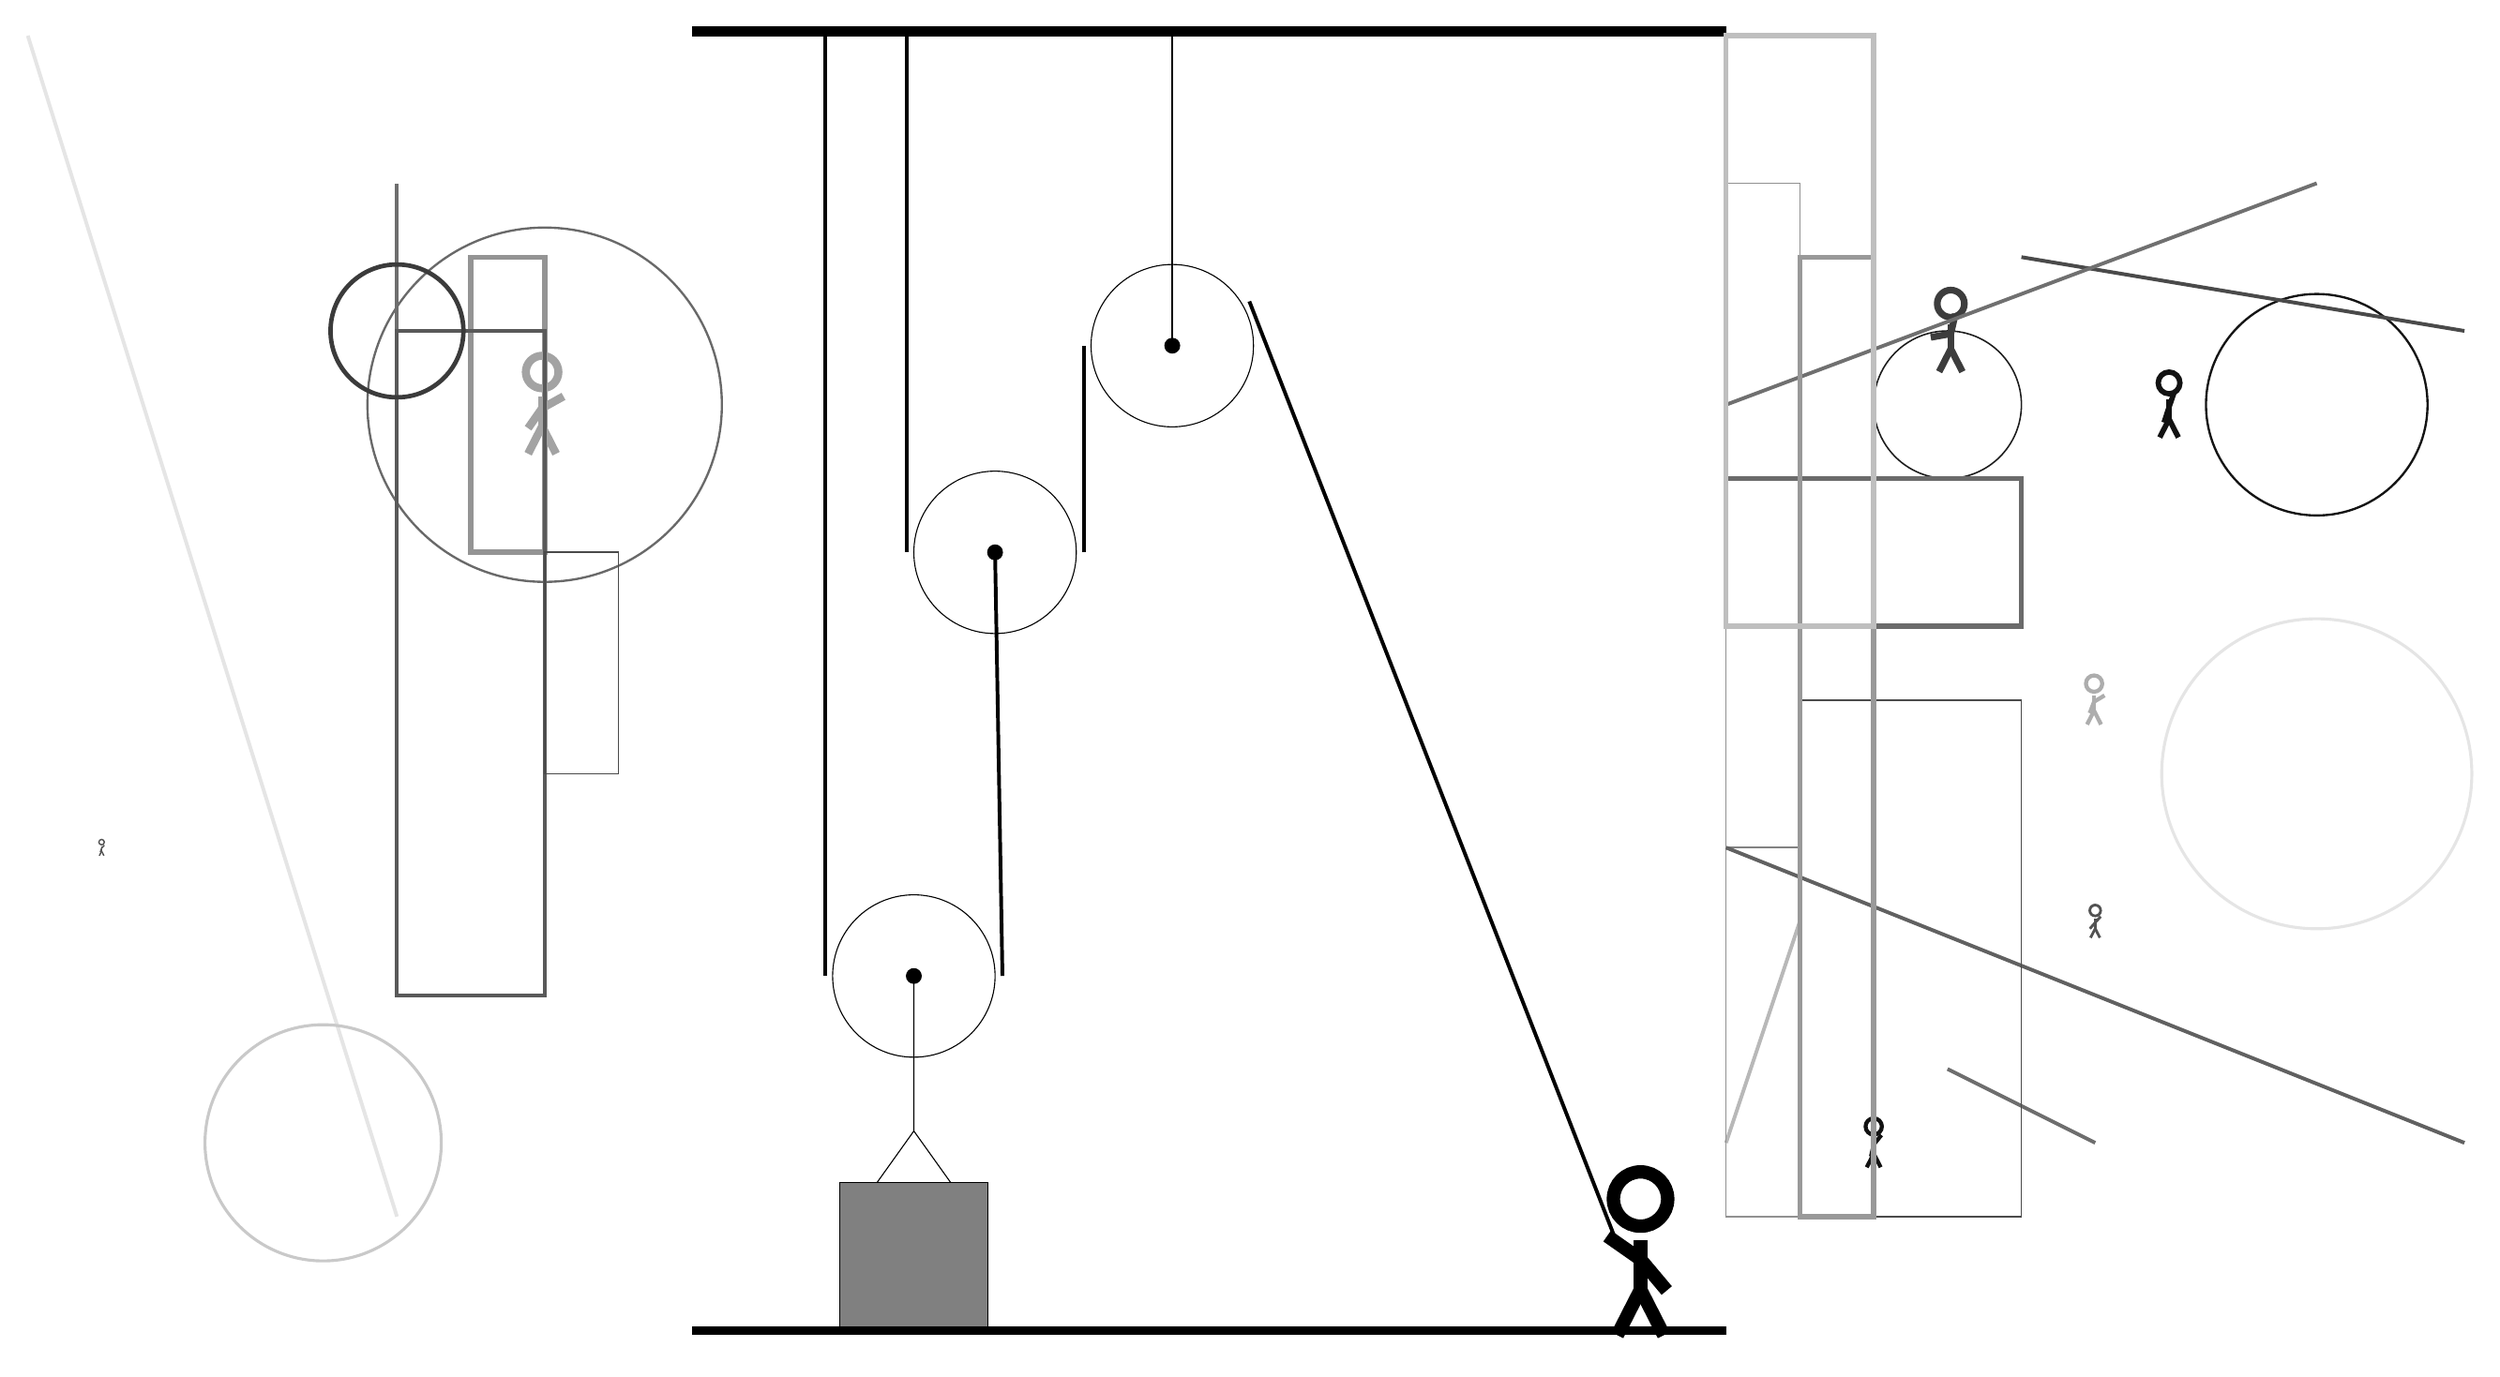
\begin{tikzpicture}
			%%%%% START %%%%%
			
			\draw[fill=black] (-2, 14) rectangle (12, 14.125);
			
			\draw [line width=0.2mm, color=black!89](15, 9) circle (1.0);
			
			\draw[line width=0.5mm, color=black!28](13, 2) -- (12, -1);
			\node[line width=0.6mm, color=black!68] at (17, 2) {\Strichmaxerl[2][49][48]};
			\draw[line width=0.5mm, color=black!10](-6, -2) -- (-11, 14);
			
			\node[line width=0.2mm, color=black!93] at (18, 9) {\Strichmaxerl[4][72][71]};
			\draw [line width=0.3mm, color=black!59](-4, 9) circle (2.4);
			\draw[line width=0.7mm, color=black!58] (12, 6) rectangle (16, 8);
			\draw [line width=0.3mm, color=black!92](20, 9) circle (1.5);
			\draw[line width=0.7mm, color=black!42] (-4, 7) rectangle (-5, 11);
			
			\node[line width=0.4mm, color=black!36] at (-4, 9) {\Strichmaxerl[6][55][29]};
			\node[line width=0.3mm, color=black!76] at (15, 10) {\Strichmaxerl[5][10][77]};
			\draw[line width=0.5mm, color=black!57](-6, 3) -- (-6, 12);
			\draw[line width=0.2mm, color=black!49] (13, 6) rectangle (12, 3);
			
			\draw[line width=0.2mm, color=black!43] (13, 12) rectangle (12, -2);
			\draw[line width=0.5mm, color=black!57](17, -1) -- (15, 0);
			\draw[line width=0.5mm, color=black!71](16, 11) -- (22, 10);
			
			\draw [line width=0.4mm, color=black!21](-7, -1) circle (1.6);
			\node[line width=0.5mm, color=black!67] at (-10, 3) {\Strichmaxerl[1][72][47]};
			\draw[line width=0.5mm, color=black!62](12, 3) -- (22, -1);
			\draw[line width=0.5mm, color=black!65] (-4, 1) rectangle (-6, 10);
			\draw[line width=0.2mm, color=black!99] (13, 0) rectangle (13, 7);
			
			\draw[line width=0.2mm, color=black!71] (13, 5) rectangle (16, -2);
			
			\draw [line width=0.4mm, color=black!10](20, 4) circle (2.1);
			\node[line width=0.3mm, color=black!93] at (14, -1) {\Strichmaxerl[3][77][51]};
			\draw [line width=0.6mm, color=black!77](-6, 10) circle (0.9);
			\draw[line width=0.5mm, color=black!56](12, 9) -- (20, 12);
			
			\draw[line width=0.2mm, color=black!71] (-3, 7) rectangle (-4, 4);
			\draw[line width=0.7mm, color=black!40] (13, 11) rectangle (14, -2);
			
			\node[line width=0.5mm, color=black!32] at (17, 5) {\Strichmaxerl[3][69][31]};
			\draw[line width=0.7mm, color=black!25] (14, 14) rectangle (12, 6);
			
			\draw (1, 1.26) circle (1.1);
			\draw[fill=black] (1, 1.26) circle (0.1);
			
			\draw (2.1, 7.0) circle (1.1);
			\draw[fill=black] (2.1, 7.0) circle (0.1);
			
			\draw (4.5, 9.8) circle (1.1);
			\draw[fill=black] (4.5, 9.8) circle (0.1);
			\draw[thick] (4.5, 9.8) -- (4.5, 14);
			
			\draw (1, 1.26) -- (1, -0.84) -- (0.5, -1.54) -- (1.5, -1.54) -- (1, -0.84);
			\draw[fill=black!50] (0, -1.54) rectangle (2, -3.54);
			
			\draw[line width=0.5mm] (-0.2, 14) -- (-0.2, 1.26);
			\centerarc[line width=0.5mm](1, 1.26)(180:360:1.2000000000000002);
			\draw[line width=0.5mm](2.2, 1.26) -- (2.1, 7.0);
			\draw[line width=0.5mm] (0.9, 14) -- (0.9, 7.0);
			\centerarc[line width=0.5mm](2.1, 7.0)(180:360:1.2000000000000002);
			\draw[line width=0.5mm](3.3, 7.0) -- (3.3, 9.8);
			\centerarc[line width=0.5mm](4.5, 9.8)(30:180:1.2000000000000002);
			\draw[line width=0.5mm] (5.544, 10.4) -- (10.5, -2.3);
			
			\node at (10.8, -2.5) {\Strichmaxerl[10][-35][-50]};
			
			\draw[fill=black] (-2, -3.5) rectangle (12, -3.6);
			
			%%%%% END %%%%%
		\end{tikzpicture}
	\end{figure}	
\end{document}